

\section{Introduksjon}

Matematikken som et teoretisk fagfelt kan løst deles inn tre deler; 
studiet av rom og former, 
studiet av endring og balanse og studiet av struktur og operasjoner. 
Det førstnevnte studiet kalles topologi, 
det andre analyse mens det siste - som vi skal lære litt om i dag - kalles algebra. 
Mer spesifikt skal vi se litt på en av de enkleste og mest kjente strukturene i denne delen av matematikk, 
nemlig det som kalles grupper. 
For å forstå disse må vi først lære litt om symmetri.  

\section{Symmetri}

Mennesker har historisk sett alltid vært utrolig interesserte i symmetri. 
Det former hva vi synes er attraktivt, 
både i andre mennesker, 
men også i kunst og natur, 
det former hva som gjør at vi kan bygge stabile bygninger vi kan leve i, 
og mye mye mer. 
Så hva er egentlig symmetri? 
En symmetri på et eller annet objekt kan defineres som en måte å rotere, 
flytte på, 
vende eller speile objektet slik at det ser helt likt ut etter på. 

Et eksempel kan være et tomt blankt ark. 
\begin{center}
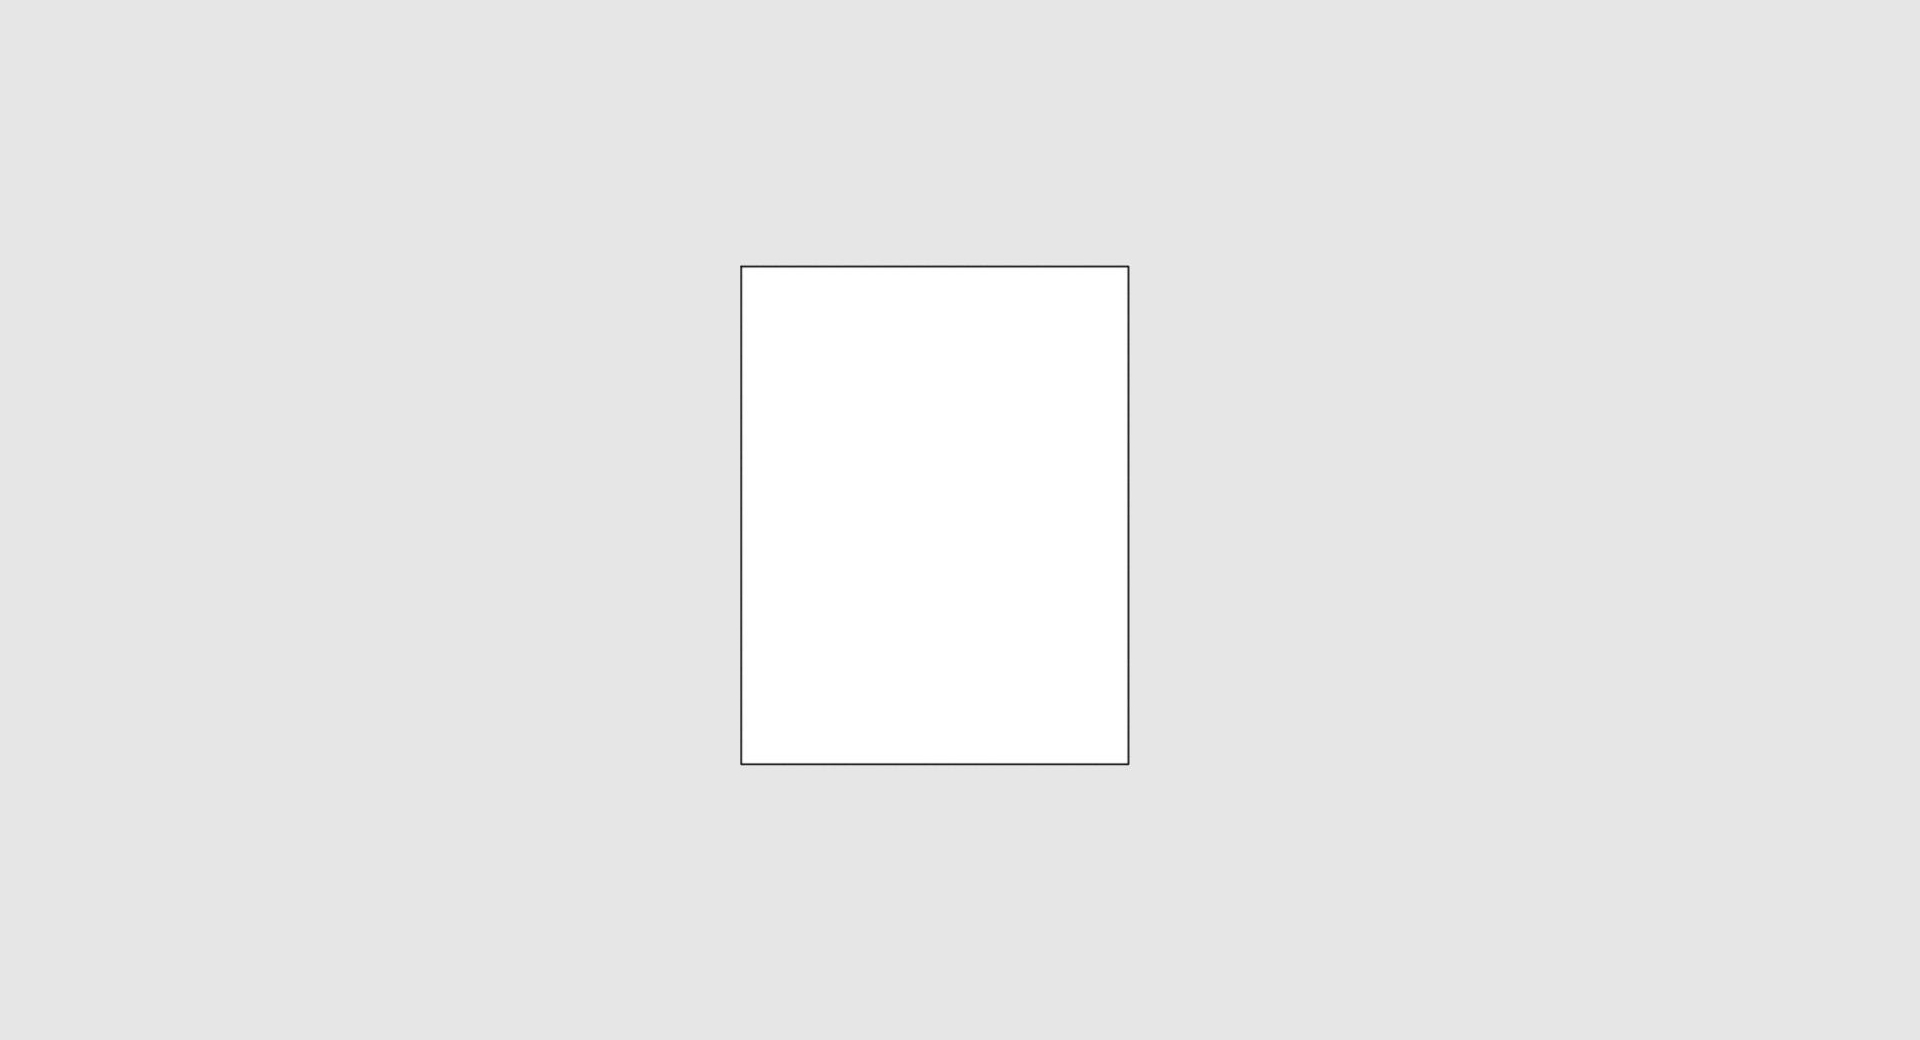
\includegraphics[width=\textwidth]{img/identity.jpg}
\end{center}

Hvordan kan vi vende, 
vri og rotere på dette arket? 
Jo vi kan for eksempel rotere arket 180 grader. 
Gjør vi dette vil arket se helt likt ut ettersom det er tomt, 
altså vet vi ikke hva som er opp eller ned på arket uten å ha noen form for markering. 
Vi kan se dette på bildet under. 
\begin{center}
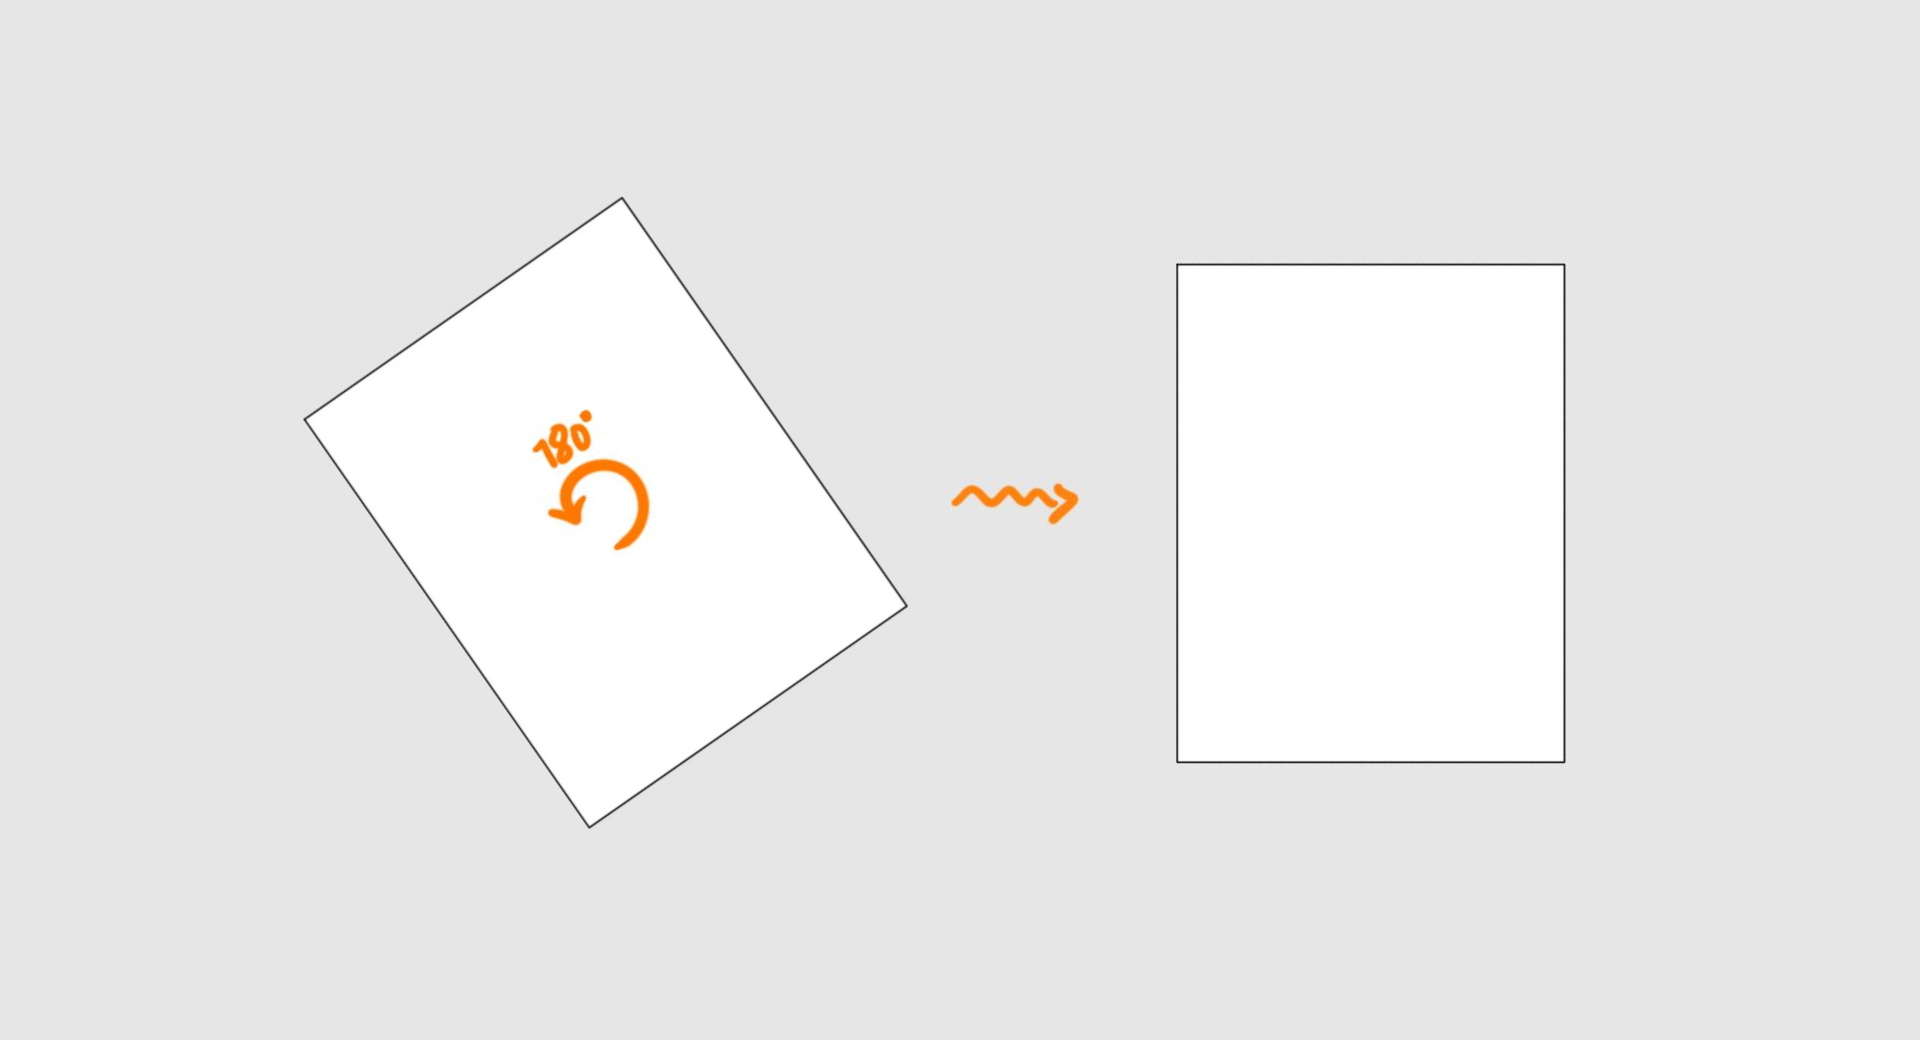
\includegraphics[width=\textwidth]{img/rotate.jpg}
\end{center}

Vi bemerker oss at det ikke har noe å si om vi roterer med eller mot klokken, 
da 180 grader begge veier vi gi den samme rotasjonen til slutt. 

Vi kan også vende arket over til den andre siden, 
og det ser fortsatt helt likt ut. 
Vi kan vende over til den andre siden på to ulike måter, 
ved å bla som en bok
\begin{center}
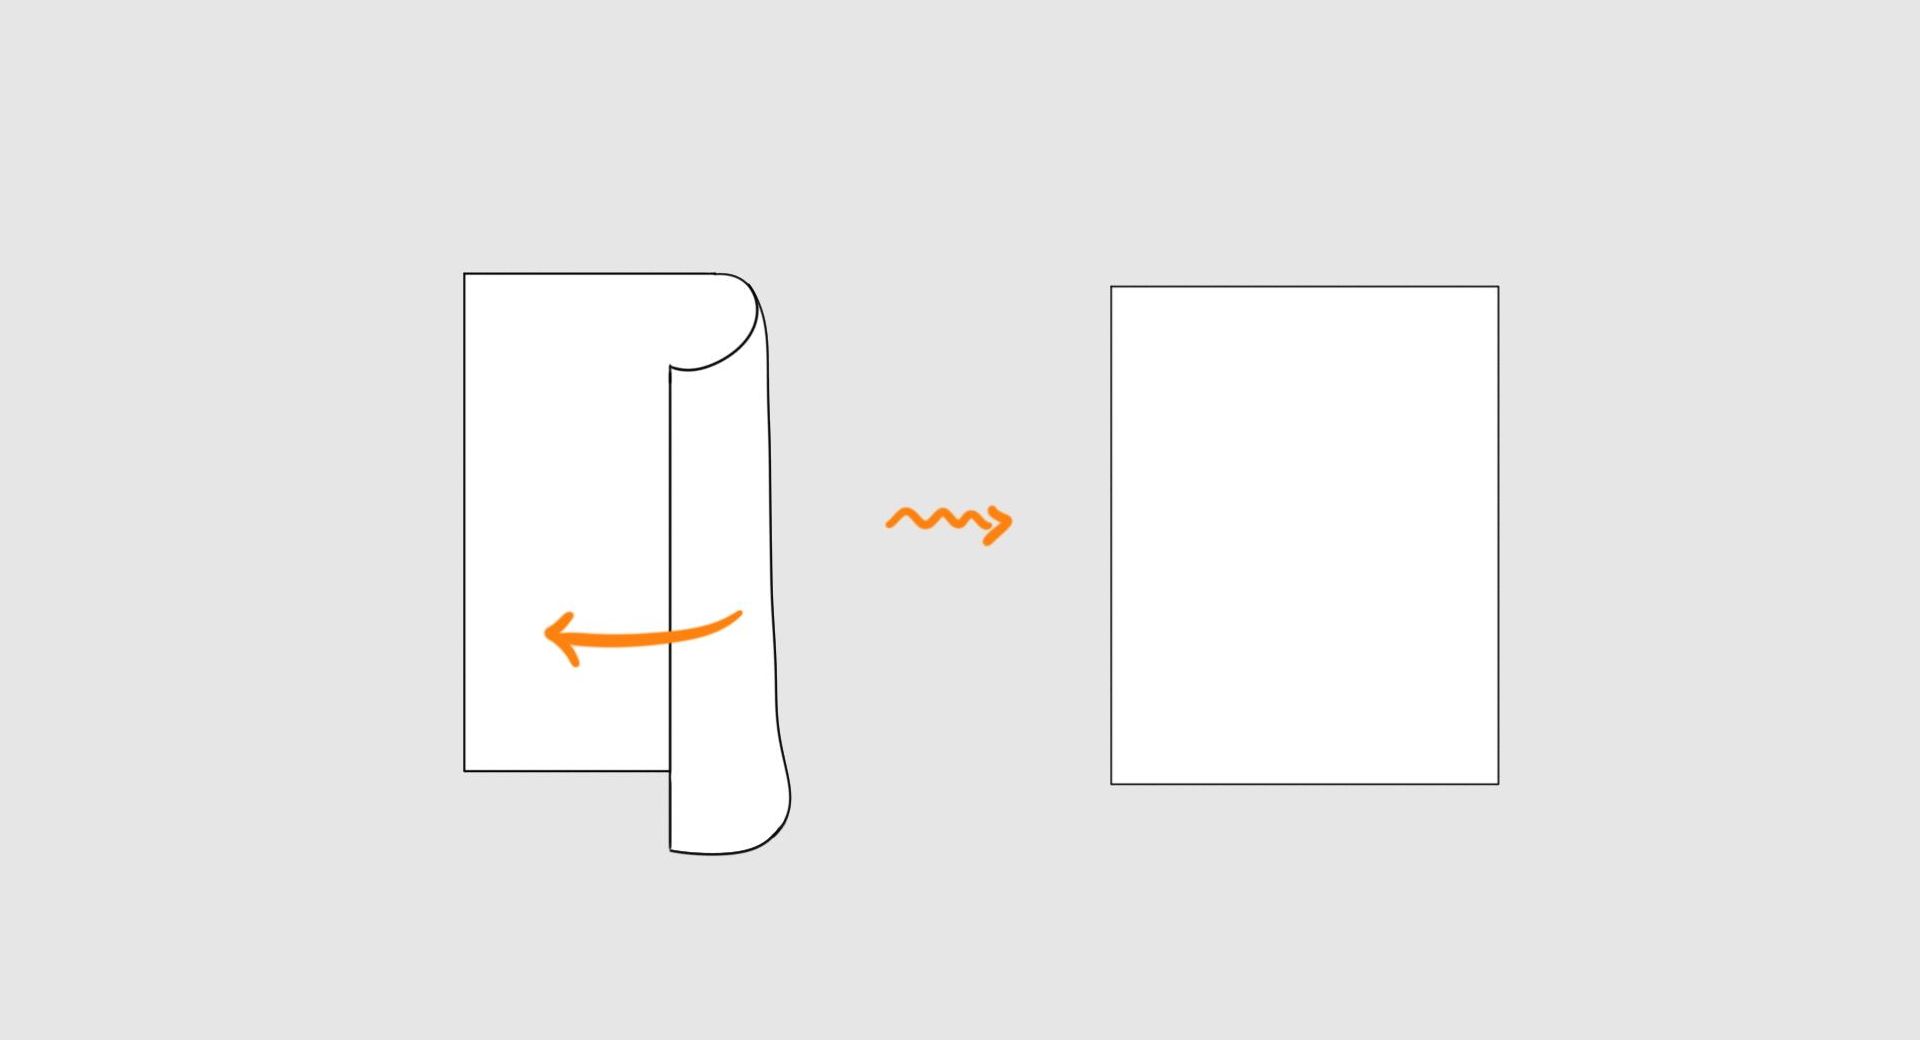
\includegraphics[width=\textwidth]{img/flip.jpg}
\end{center}

eller ved å bla oppover som i noen tegneblokker
\begin{center}
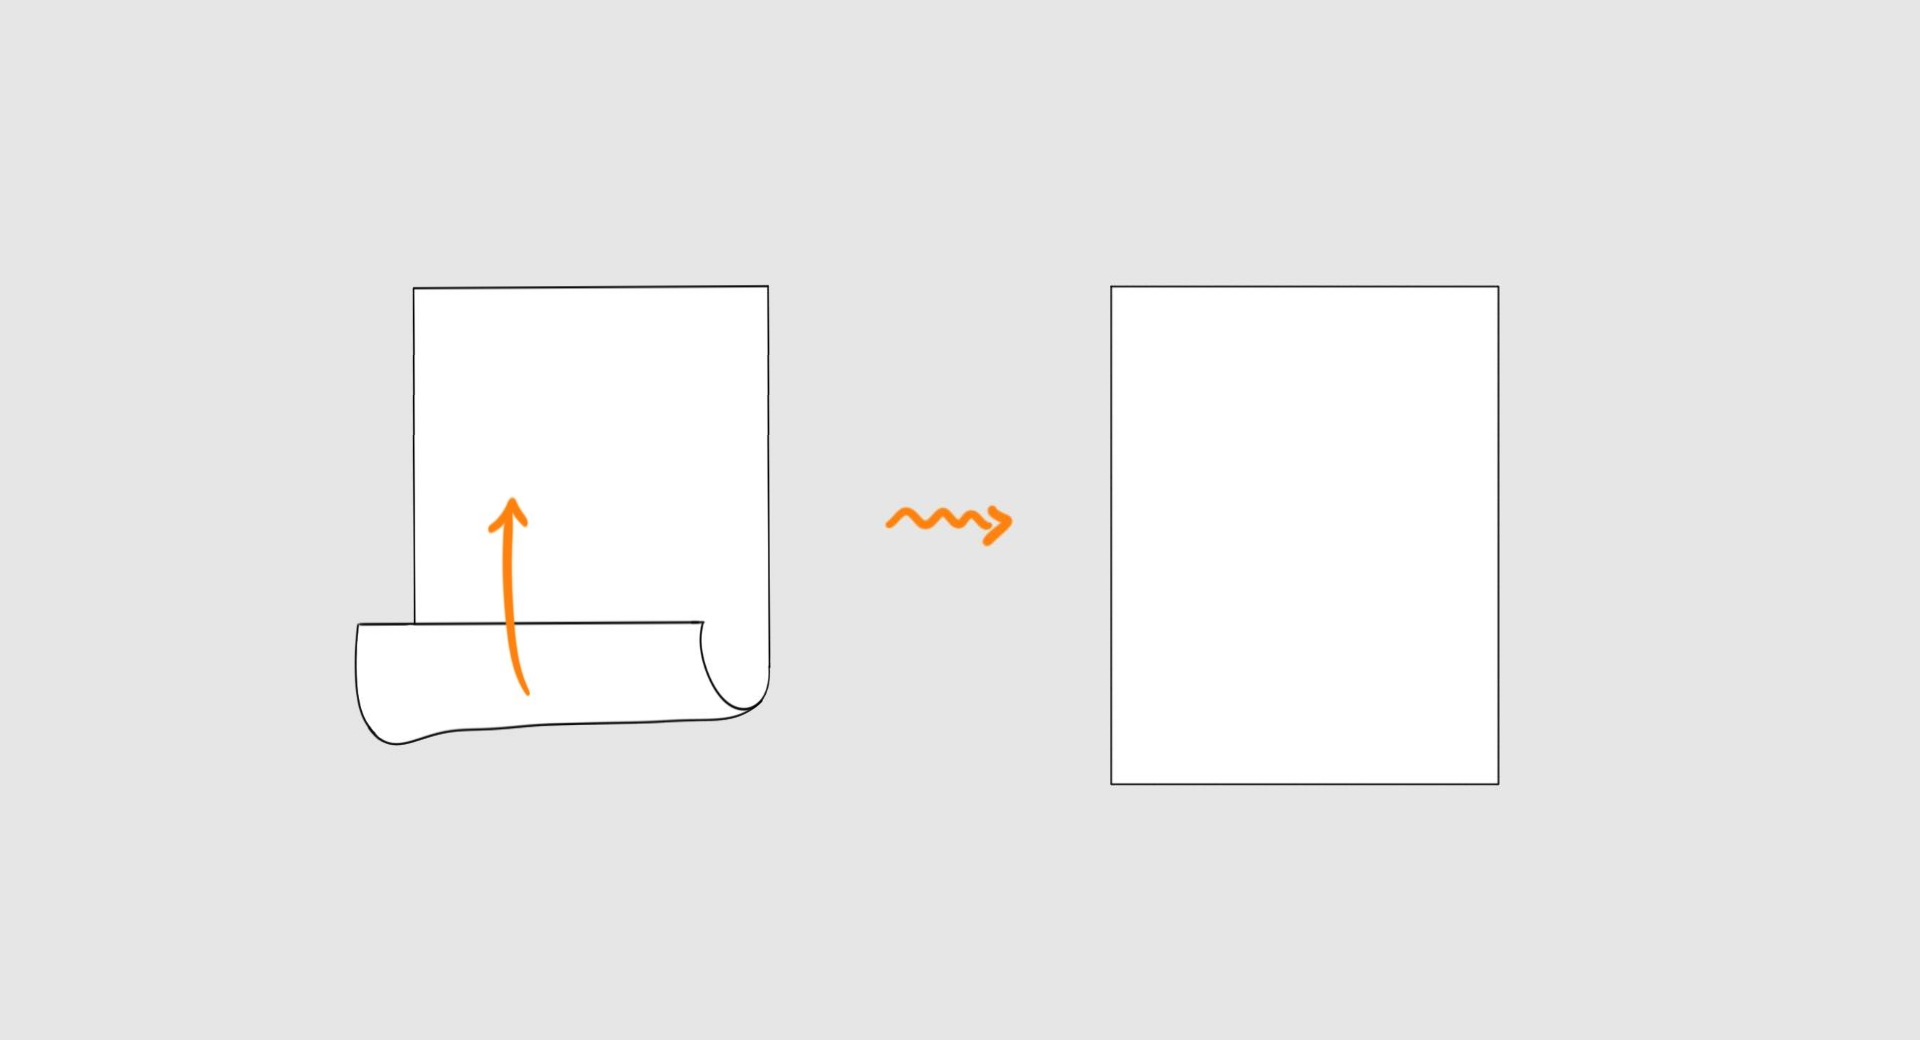
\includegraphics[width=\textwidth]{img/flip2.jpg}
\end{center}

I likhet med rotasjonen bemerker vi oss at det ikke har noe å si hvilken vei vi blar. 
Å bla til høyre eller til venstre vil gi samme resultat, 
og det samme med opp eller ned. 

Disse er de tre symmetriene et blankt ark har hvis vi kun kan bruker fysiske rotasjoner og vendinger. 
For eksempel speiling over midtlinjen vill også være en symmetri, 
men i dette eksemplet teller vi ikke med disse da de ikke kan fysisk utføres på arket. 
For å gjøre det litt enklere for oss selv kaller til å vende arket som en bok for horisontal vending, 
og bla arket som en tegneblokk for vertikal vending. 

En utrolig viktig egenskap med disse symmetriene er at vi kan kombinere dem. 
For eksempel kan vi først vende arket horisontalt, 
og så rotere med 180 grader. 
Men hvis man prøver dette så ser man at de to etterfulgt av hverandre er det samme som å vende arket vertikalt. 
Dette skjer også med de andre kombinasjonene av symmetrier vi kan gjøre. 
For eksempel så er en vertikal vending etterfulgt av en horisontal vendig det samme som å rotere arket 180 grader. 
Dermed får vi at å kombinere to symmetrier, 
altså å gjøre de etter hverandre også er en symmetri! 
Siden vi også kan gjøre symmetriene baklengs, 
altså å vende i den andre retningen kan vi også altid komme oss tilbake til startposisjonen vår. 
Altså vil en rotasjon etterfulgt av enda en rotasjon føre oss tilbake der vi startet. 
Det samme skjer for de to vendingene. 

\section{Grupper}

Så hva er egentlig en gruppe, 
og hva har det med disse symmetriene å gjøre? 
En gruppe kan defineres som samlingen av symmetrier på et objekt, 
der vi har muligheten for å legge de sammen, 
altså gjøre de etter hverandre. 
For å gjøre det litt bedre må vi ha muligheten til å gjøre alle symmetriene våre baklengs, 
altså reversere de, 
og at å gjøre symmetriene etter hverandre på forskjellige måter ikke endrer resultatet. 

Du tenker kanskje at dette er veldig elementært og at dette ikke er matematikk i det hele tatt, 
men vi kan nå begynne å se på dette konseptet på en matematisk måte. 

La oss nå bruke symboler for å beskriver symmetriene istedet. 
Vi fortsetter å bruke eksemplet fra tidligere. 
La symbolet $1$ bety at vi er ved startposisjonen. 
Vi lar $r$ bety rotasjon med 180 grader, 
$h$ bety horisontal vending og 
$v$ bety vertikal vending. 
Vi lar også $-r$ bety å rotere baklengs, 
og det samme for $-h$ og $-v$. 
Siden det i eksempelet vårt er tilfelle at rotasjon med og mot klokken er det samme og at begge vendingene baklengs også er det samme, 
får vi at $-r=r$, 
$-h=h$ og $-v=v$. 
Hvis vi nå begynner å kombinere disse som tidligere får vi $r+r=1$, 
$h+h=1$ og $v+v=1$. 
Dette er fordi vi kommer tilbake til startposisjonen etter å gjøre de to ganger, 
slik som beskrevet tidligere. 
Hvis vi kombinerer ulike symmetrier får vi $r+v=h$, 
$v+r=h$, 
$r+h=v$, 
$h+r=v$, 
$v+h=r$ og $h+v=r$. 
Disse er alle kombinasjonene vi kan gjøre. 

Vi kan gjøre eksempelet litt mer interessant ved å bruke et kvadratisk papir i steden for det rektangulære.

\begin{center}
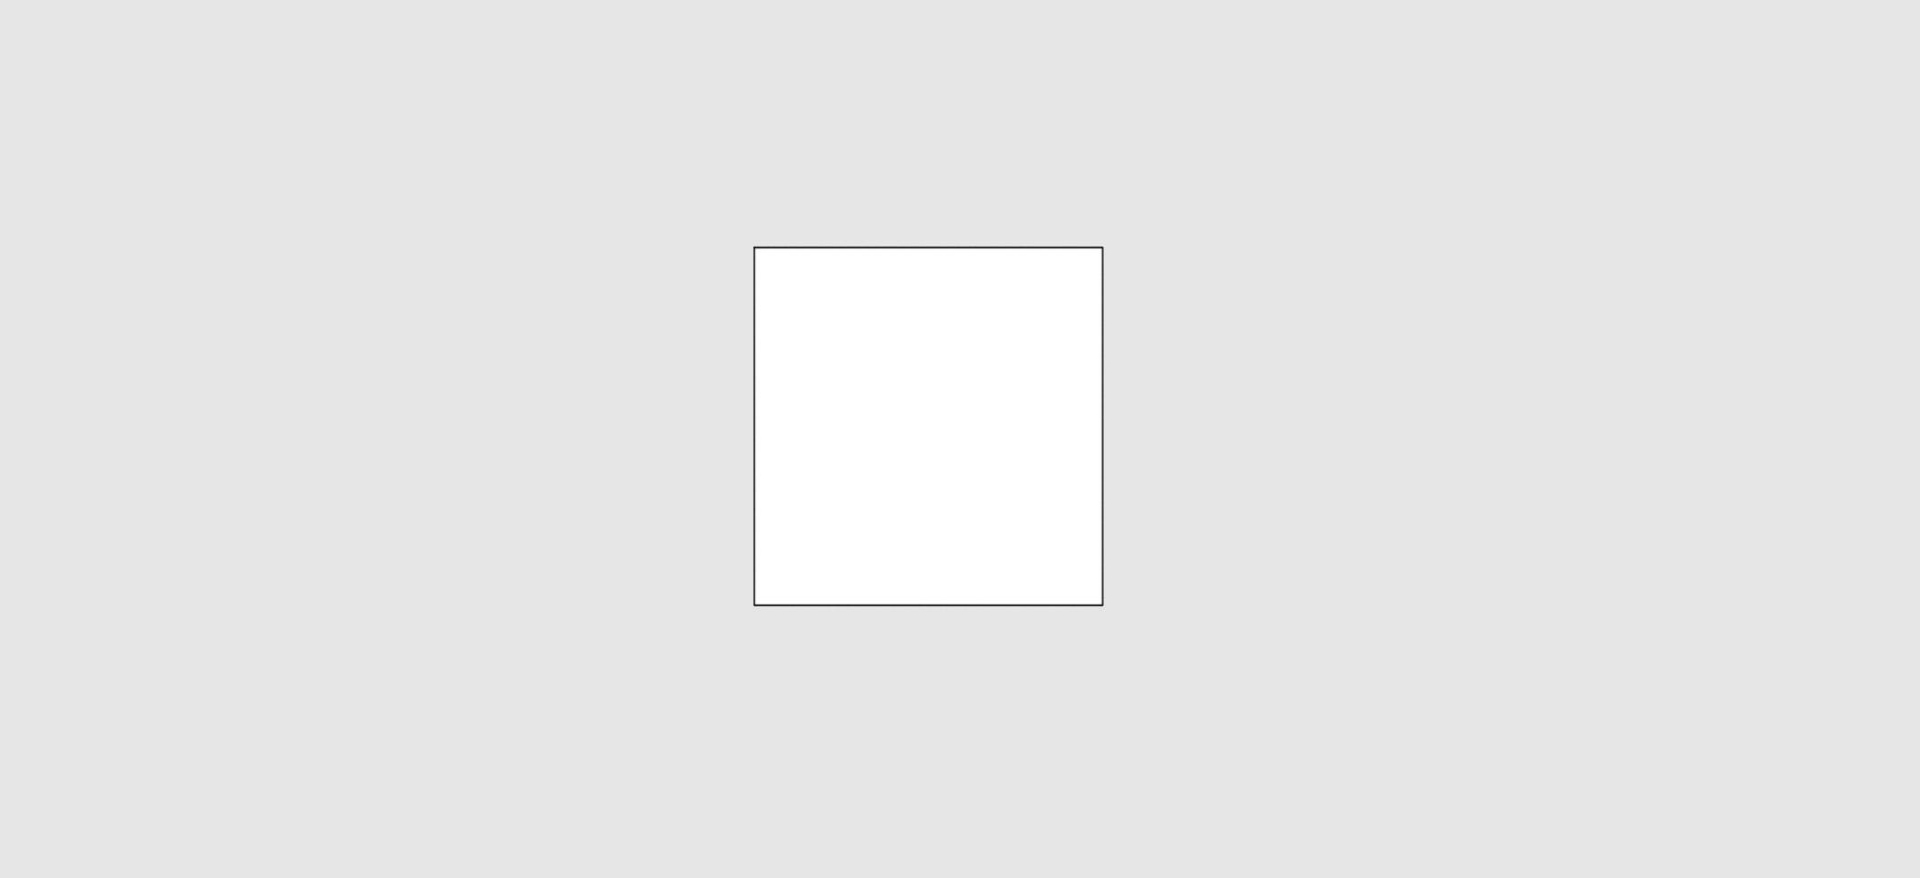
\includegraphics[width=\textwidth]{img/identity2.jpg}
\end{center}

Nå ser vi at vi i tillegg til de rotasjonene og vendingene vi hadde tidligere for det rektangulære papiret, 
har vi at å rotere med 90 grader også er en symmetri. 
Vi lar fortsatt $r$ betegne rotasjon, 
men nå rotasjon med 90 grader mot klokken i steden for 180 grader. 
Dermed har vi $r+r+r+r=3r=1$ istedenfor, 
ettersom vi må rotere fire ganger for å komme tilbake der vi startet. 
Nå er heller ikke det å rotere mot eller med klokken det samme lengre. 
Men, vi ser at å rotere 90 grader med klokken er det samme som å rotere 90 grader mot klokken tre ganger. 
Siden å rotere med klokken tilbakegjør det å rotere mot klokken skriver vi $-r = 3r$. 

Vi kan nå også vende arket om de to diagonalene, 
noe som skaper to nye ny symmetrier som vi kaller $n$ og $\o$. 
Den nedre diagonalen $n$ går fra hjørnet nederst til venstre opp til hjønet oppe til høyre, 
mens den øvre, $\o$, 
går fra hjørnet øverst til venstre ned til hjørnet nede til høyre. 
Under ser man en vending om den øvre diagonalen, 
alstå symmetrien $\o$.  

\begin{center}
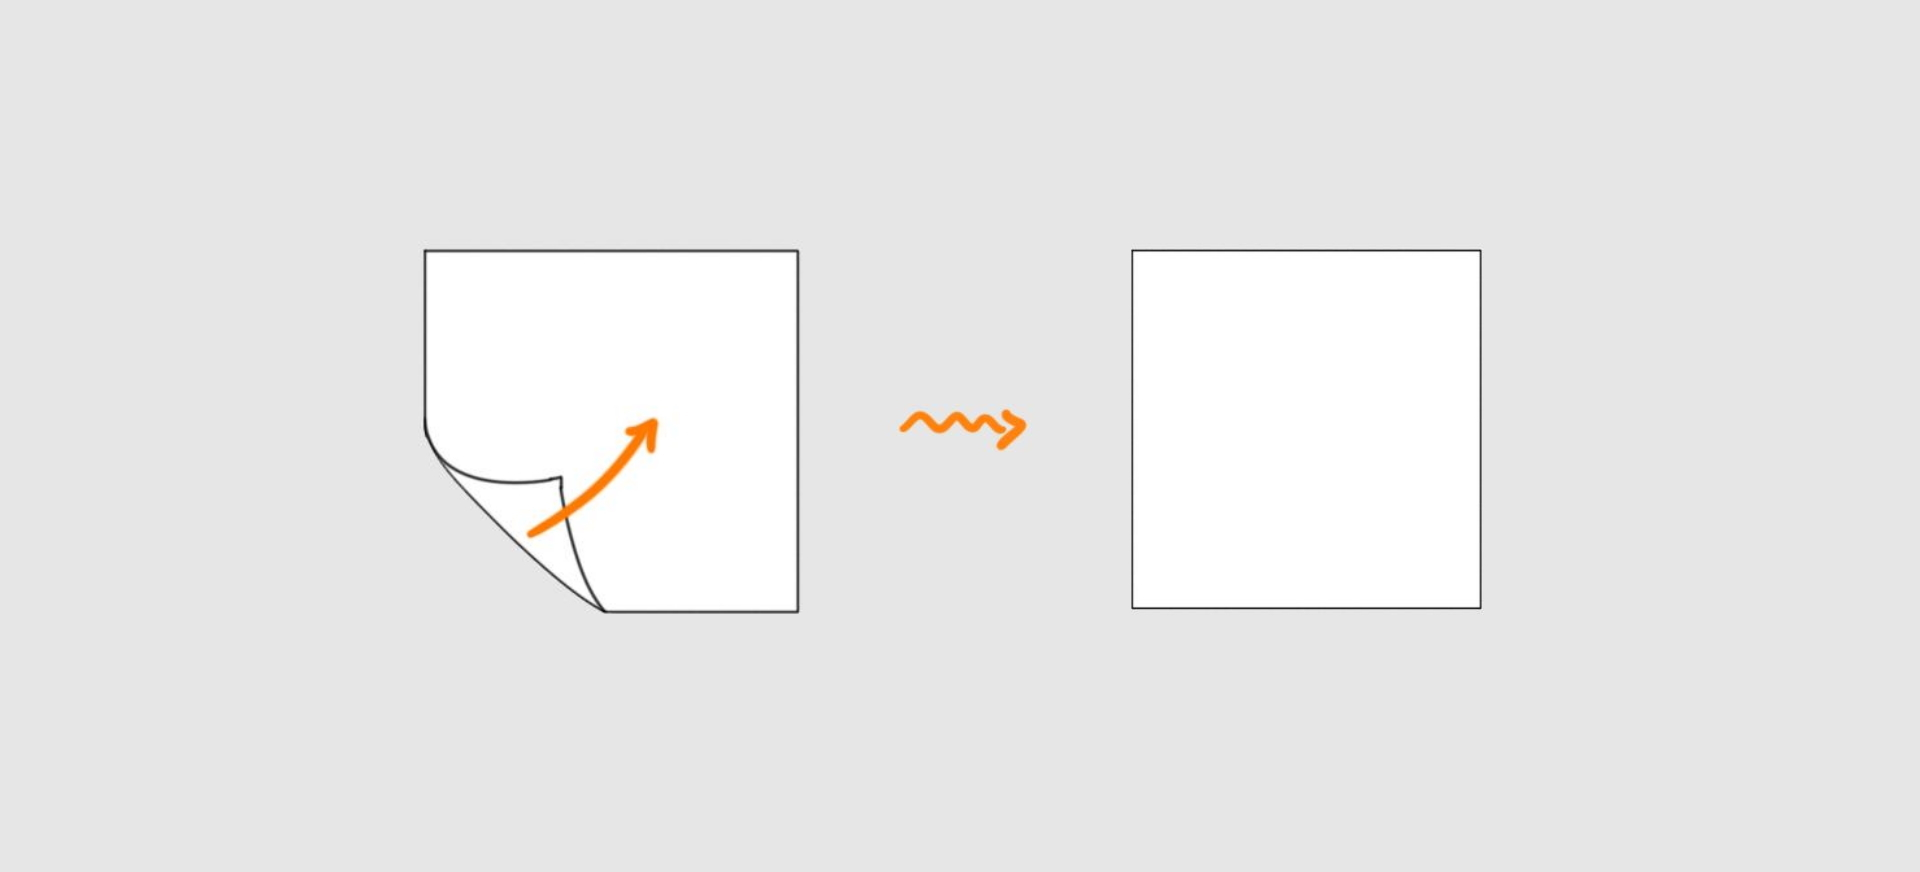
\includegraphics[width=\textwidth]{img/diagonal.jpg}
\end{center}

Vi har nå også noen nye kombinasjoner av symmetrier som vi ikke hadde tidligere. 
For eksempel er nå $r+h = n$ og $h+r=\o$. 

Altså har et kvadrat flere symmetrier en et rektangel, 
noe som gir mening. 

Vi avslutter denne lille undervisningen med den matematiske rigorøse definisjonen av en gruppe. 

\begin{definition}{Gruppe}
En gruppe er en mengde $G$ sammen med en binæroperasjon $m:G\times G\rightarrow G$ slik at 
\begin{itemize}
    \item $m$ er assosiativ
    \item det finnes et element $1\in G$ slik at $m(g,1)=g=m(1,g)$ for alle elementer $g\in G$
    \item for alle elementer $g\in G$ finnes det et annet element, som vi skriver som $-g$, slik at $m(g, -g)=1$
\end{itemize}
\end{definition}

I eksemplene våre tidligere var $G$ definert til å være samlingen av symmetrier på et rektagel, 
eller et kvadrat. 
Elementet $1$ var definert til å være symmetrien som ikke gjorde noe, 
altså startposisjonen vår. 
Vi definerte operasjonen $m$ til å være ``etterfulgt av'' altså å gjøre symmetriene etter hverandre, 
og elementet $-g$ var å gjøre symmetrien baklengs. 
At operasjonen er assosiativ betyr bare at å gjøre operasjonene etter hverandre på ulike måter ikke endrer resultatet, 
altså at å bruke paranteser ikke har noen effekt på selve symmetriene. 
Matematisk beskrives dette som $r+(h+v)=(r+h)+v$. 

Dermed var faktisk samlingen av symmetrier på et objekt en gruppe! 
Det viser seg også gjennom litt avansert gruppeteori at alle grupper kan ses på som symmetriene til et eller annet objekt. 
Dette er omtalt som Cayleys teorem. 

